\chapter{Visualizing Dynamic Input Graphs}
\label{chap:visualizing-dynamic-input-graphs}

Extending the approach discussed in the previous section to dynamic input graphs is challenging primarily because we must try to preserve the viewer's mental map as the underlying data changes over time. We want the visualization at different points in time to be similar enough so that the viewer can clearly tell what parts have changed \cite{mashima2011visualizing}, yet allow for the required changes in geography and topology. Still, changes between visualizations at consecutive points in time should minimize movement and allow for smooth animations therebetween.

The pipeline for static inputs discussed in the previous section does not satisfy these requirements. Running through the entire pipeline with a different, albeit similar, input graph, may result in a completely different visualization, destroying the viewer's mental map. We therefore extend the pipeline in a way that allows for small, incremental changes to be propagated through the pipeline and to eventually be applied to the previous output in a way that preserves the viewer's mental map.

We extend the pipeline for static input by an incremental transformation phase. This phase takes two inputs: A proportional map graph $G_\text{prop}$ that the pipeline previously produced as output for some cluster graph $G_\text{emb}$, and a sequence of operations on said cluster graph, that, when applied to $G_\text{emb}$, yields the cluster graph $G_\text{emb}^\prime$. The incremental embedding phase then determines how these operations translate to a polygonal dual of $G_\text{emb}$ and applies the translated operations to $G_\text{prop}$, producing $G_\text{init}^\prime$, a (not necessarily approximately area-proportional) polygonal dual of $G_\text{emb}^\prime$. This polygonal dual is then fed back into the drawing phase to make it approximately area-proportional and improve the local fatness of the map's regions.

\begin{figure}[H]
	\centering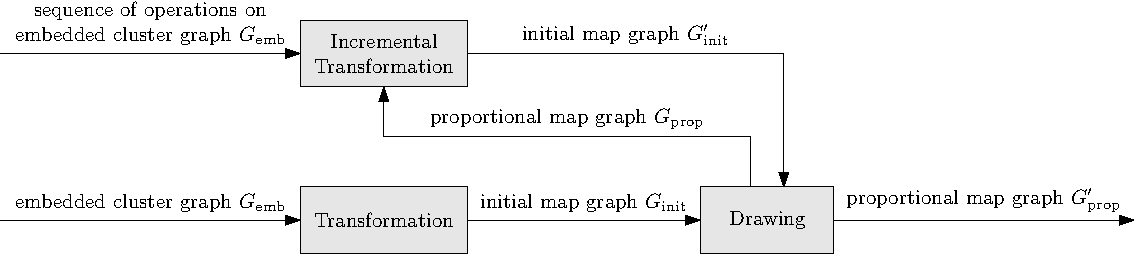
\includegraphics[width=0.9\textwidth]{Resources/Pipeline-Thesis-Dynamic.pdf}
	\caption{Overview of the algorithmic pipeline for dynamic input graphs.}
	\label{fig:dynamic-pipeline-thesis}
\end{figure}

Real-world applications such as visualizing a dynamic opinion network need a way to feed a sequence of operations on the embedded cluster graph into our framework. This could be done by prepending an incremental clustering phase that translates changes to the simple input graph into changes of its embedded cluster graph. However, such a sequence of operations is only meaningful in combination with a graph that these operations can be applied to. One must provide the previously-produced cluster graph as additional input to the incremental clustering phase such that it can tailor its output to the cluster graph that has already been locked in in an earlier run through the pipeline.

This tweak to our pipeline is illustrated in the following figure:
%
\begin{figure}[H]
	\centering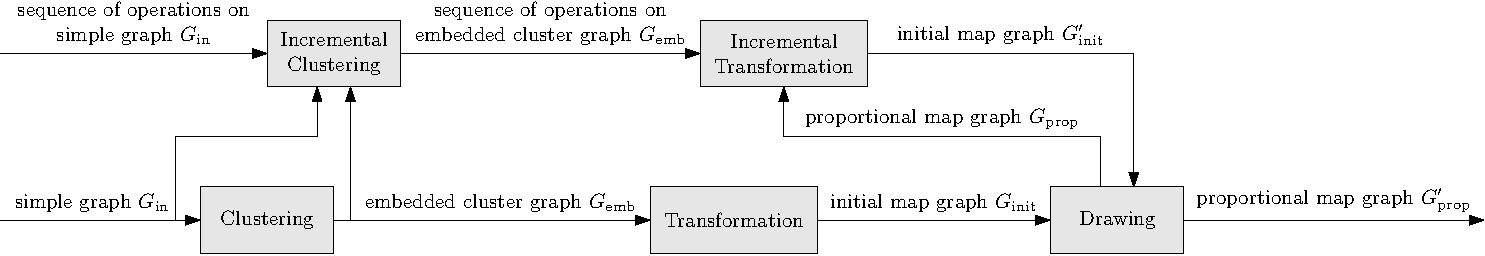
\includegraphics[width=0.9\textwidth]{Resources/Pipeline-Application-Dynamic.pdf}
	\caption{Overview of a possible algorithmic pipeline for generic applications.}
	\label{fig:dynamic-pipeline-application}
\end{figure}

Extending the pipeline to allow the propagation of small, incremental changes of the input graph has numerous benefits other than the ability to preserve the viewer's mental map:
%
\begin{itemize}
	\item It allows highly efficient implementations of the incremental parts of the pipeline as only the aspects that have actually changed in the input graph or intermediate products need to be processed and propagated further along the pipeline.
	\item It makes the dynamic pipeline highly parallelizable: when a later phase is processing changes, an earlier phase can already start processing new changes independently. With our force-directed implementation of the drawing phase, we can even incorporate dynamic updates while the drawing phase is still running, even if it has not converged yet: we pause the force simulation, feed the current map graph $G_\text{prop}$ into the incremental transformation phase to incorporate the dynamic updates, and then resume the simulation with the updated map graph $G_\text{init}^\prime$ produced by the incremental transformation phase.
	\item It efficiently supports dynamic input in an online setting, \ie{} a setting in which the incremental changes aren't known in advance, for example when visualizing live data.
\end{itemize}

\clearpage
\todo{Just listing these operations here and having implementation right afterwards doesn't seem make sense. How about just listing names, inline, in text, and saying in the following sections, we look at these operations in detail: what preconditions, and how to apply?}
Our pipeline supports the following classes of primitive operations on the cluster graph:
%
\begin{itemize}
	\item \textbf{Update vertex weight:} Obviously, we can set existing vertices' weights to arbitrary new values.

	\item \textbf{Insert vertex in an internal face:} We can place a new vertex with arbitrary weight inside one of the internal faces (which are triangles). In order to preserve the internal triangulatedness of the graph, edges to the three vertices on said face must be added in conjunction and the edges must be embedded such that they do not cross. This operation essentially replaces an internal face with three new triangles.
\begin{figure}[H]
	\centering
	\subfigure[]{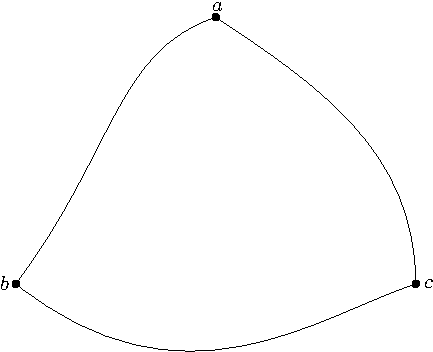
\includegraphics[height=30mm]{Resources/IncrementalFilteringAndEmbedding-InsertVertexInside-Initial.pdf}}
	\quad
	\subfigure[]{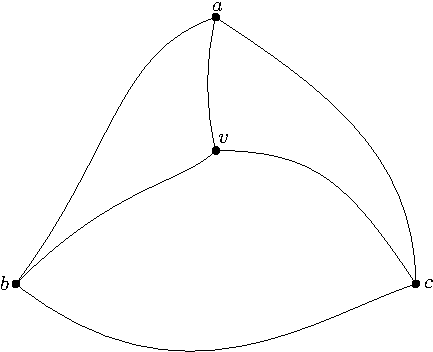
\includegraphics[height=30mm]{Resources/IncrementalFilteringAndEmbedding-InsertVertexInside-Valid.pdf}}
	\quad
	\subfigure[]{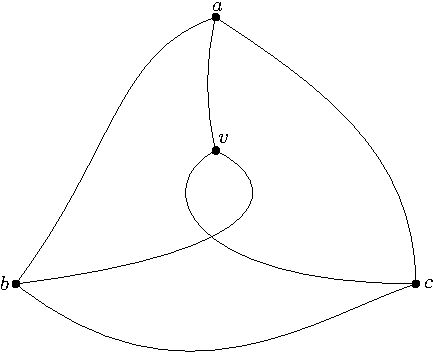
\includegraphics[height=30mm]{Resources/IncrementalFilteringAndEmbedding-InsertVertexInside-Invalid.pdf}}
	\caption{Inserting a vertex in an internal face of a embedded filtered graph (a) correctly (vertex $v$, b) and incorrectly, introducing a crossing of the edges $\{b,v\}$, $\{c,v\}$ (vertex $v$, c).}
	\label{fig:transformation}
\end{figure}

	\item \textbf{Insert vertex in outer face:} We can also place a new vertex with arbitrary weight inside the outer face. The new vertex must be connected to at least two vertices on the outer face (to preserve 2-connectivity), and its adjacent vertices must form a simple path along the original outer face (to preserve internal triangulatedness).
\begin{figure}[H]
	\centering
	\subfigure[]{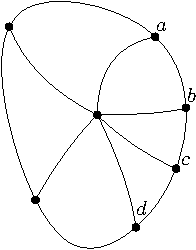
\includegraphics[height=30mm]{Resources/IncrementalFilteringAndEmbedding-InsertVertexOutside-Initial.pdf}}
	\quad
	\subfigure[]{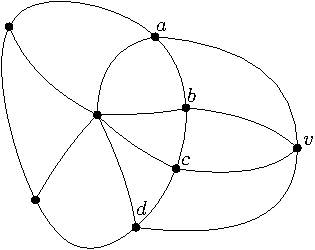
\includegraphics[height=30mm]{Resources/IncrementalFilteringAndEmbedding-InsertVertexOutside-Valid.pdf}}
	\quad
	\subfigure[]{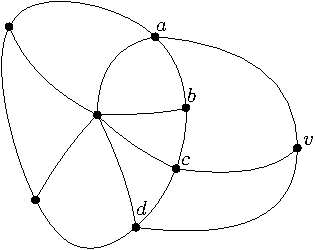
\includegraphics[height=30mm]{Resources/IncrementalFilteringAndEmbedding-InsertVertexOutside-Invalid.pdf}}
	\caption{Inserting a vertex in the outer face of an embedded filtered graph (a) correctly (vertex $v$, b) and incorrectly, creating a 4-hole $abcv$ (vertex $v$, c).}
	\label{fig:transformation}
\end{figure}

	\clearpage
	\item \textbf{Remove internal vertex:} We can only remove internal vertices along with their incident edges if they have degree 3. Such vertices are incident to three pairwise incident triangular faces and their removal would fuse the three triangles together to form a new triangular face.
\begin{figure}[H]
	\centering
	\subfigure[]{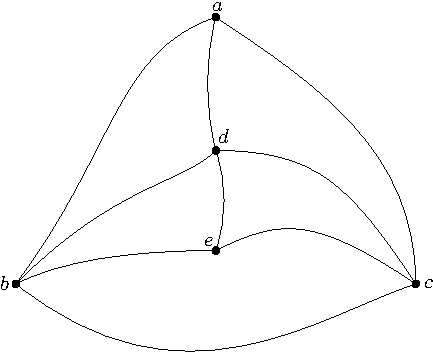
\includegraphics[height=30mm]{Resources/IncrementalFilteringAndEmbedding-RemoveInternalVertex-Initial.pdf}}
	\quad
	\subfigure[]{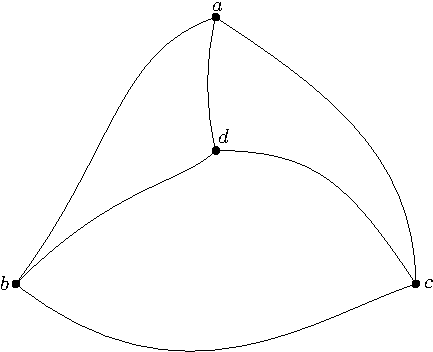
\includegraphics[height=30mm]{Resources/IncrementalFilteringAndEmbedding-RemoveInternalVertex-Valid.pdf}}
	\quad
	\subfigure[]{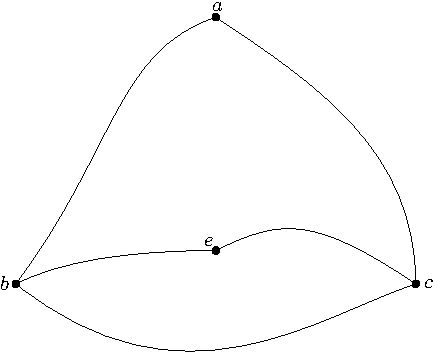
\includegraphics[height=30mm]{Resources/IncrementalFilteringAndEmbedding-RemoveInternalVertex-Invalid.pdf}}
	\caption{Removing an internal vertex of an embedded filtered graph (a) correctly (vertex $e$, b) and incorrectly, creating a 4-hole $abec$ (vertex $d$, c).}
	\label{fig:transformation}
\end{figure}

	\item \textbf{Remove vertex on outer face:} Vertices on the outer face can be removed along with their incident edges as long as the resulting graph remains 2-connected.
\begin{figure}[H]
	\centering
	\subfigure[]{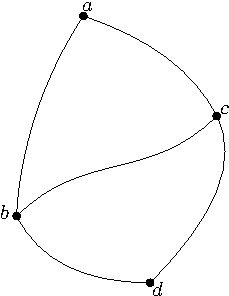
\includegraphics[height=30mm]{Resources/IncrementalFilteringAndEmbedding-RemoveOuterVertex-Initial.pdf}}
	\quad
	\subfigure[]{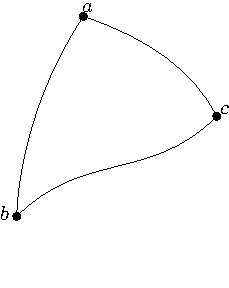
\includegraphics[height=30mm]{Resources/IncrementalFilteringAndEmbedding-RemoveOuterVertex-Valid.pdf}}
	\quad
	\subfigure[]{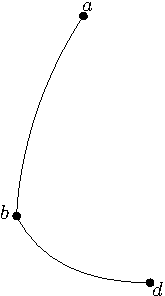
\includegraphics[height=30mm]{Resources/IncrementalFilteringAndEmbedding-RemoveOuterVertex-Invalid.pdf}}
	\caption{Removing a vertex on the outer face of an embedded filtered graph (a) correctly (vertex $d$, b) and incorrectly, creating a cut vertex $b$ (vertex $c$, c).}
	\label{fig:transformation}
\end{figure}

	\item \textbf{Flip internal edge:} Internal edges $\{u, v\}$ can be flipped unless their two incident triangles \quoted{tips} $w, x$ are already adjacent. This operation replaces the edge $\{u, v\}$ with the edge $\{w, x\}$ and would therefore create an unwanted duplicate adjacency if $w$ and $x$ were already adjacent.
\begin{figure}[H]
	\centering
	\subfigure[]{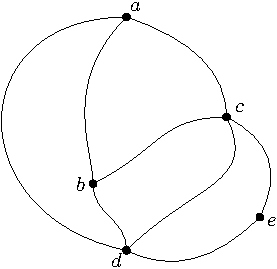
\includegraphics[height=30mm]{Resources/IncrementalFilteringAndEmbedding-FlipInternalEdge-Initial.pdf}}
	\quad
	\subfigure[]{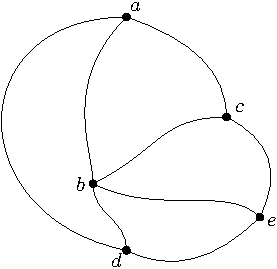
\includegraphics[height=30mm]{Resources/IncrementalFilteringAndEmbedding-FlipInternalEdge-Valid.pdf}}
	\quad
	\subfigure[]{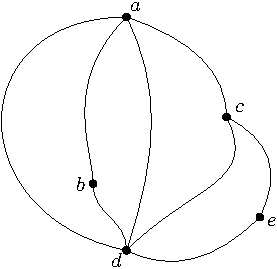
\includegraphics[height=30mm]{Resources/IncrementalFilteringAndEmbedding-FlipInternalEdge-Invalid.pdf}}
	\caption{Flipping an internal edge of an embedded filtered graph (a) correctly (edge $\{d,c\}$, b) and incorrectly, creating a duplicate adjacency between $a$ and $d$ (edge $\{b,c\}$, c).}
	\label{fig:transformation}
\end{figure}

	\clearpage
	\item \textbf{Insert edge on outer face:} Edges between nonadjacent vertices $u, v$ on the outer face may only be inserted if they preserve the graph's internal triangulatedness, \ie{} they don't create holes in the graph. Adding such an edge creates a new internal face and is therefore only possible iff $u$ and $v$ have a neighbor in common.
\begin{figure}[H]
	\centering
	\subfigure[]{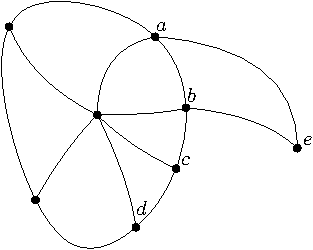
\includegraphics[height=30mm]{Resources/IncrementalFilteringAndEmbedding-InsertOuterEdge-Initial.pdf}}
	\quad
	\subfigure[]{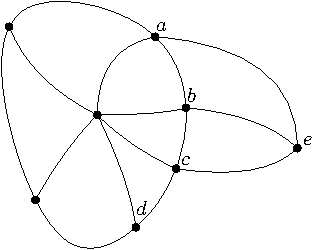
\includegraphics[height=30mm]{Resources/IncrementalFilteringAndEmbedding-InsertOuterEdge-Valid.pdf}}
	\quad
	\subfigure[]{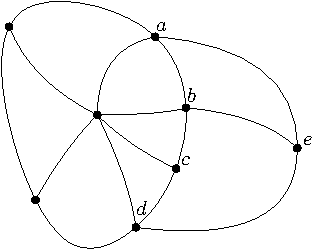
\includegraphics[height=30mm]{Resources/IncrementalFilteringAndEmbedding-InsertOuterEdge-Invalid.pdf}}
	\caption{Inserting an edge on the outer face of an embedded filtered graph (a) correctly (edge $\{e,c\}$, b) and incorrectly, creating a 4-hole $bcde$ ($\{e,d\}$, c).}
	\label{fig:transformation}
\end{figure}

	\item \textbf{Remove edge on outer face:} Similarly, we can remove an edge $\{u, v\}$ on the outer face only if it doesn't create holes in the graph. This is the case iff $u$ and $v$ share a neighbor. The graph must also remain 2-connected.
\begin{figure}[H]
	\centering
	\subfigure[]{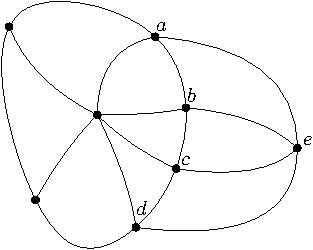
\includegraphics[height=30mm]{Resources/IncrementalFilteringAndEmbedding-RemoveOuterEdge-Initial.pdf}}
	\quad
	\subfigure[]{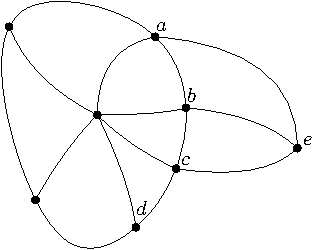
\includegraphics[height=30mm]{Resources/IncrementalFilteringAndEmbedding-RemoveOuterEdge-Valid.pdf}}
	\quad
	\subfigure[]{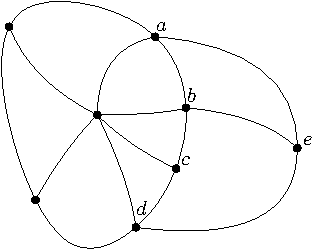
\includegraphics[height=30mm]{Resources/IncrementalFilteringAndEmbedding-RemoveOuterEdge-Invalid.pdf}}
	\caption{Removing an edge on the outer face of an embedded filtered graph (a) correctly (b, edge $\{e,d\}$) and incorrectly, creating a 4-hole $bcde$ (edge $\{e,c\}$, c).}
	\label{fig:transformation}
\end{figure}
\end{itemize}

In the following discussion of our implementation of the incremental transformation phase, we will see how these operations can be applied to an existing map graph.

\clearpage
\section{Incremental Transformation to Polygonal Dual}
\label{sect:incremental-transformation-to-dual}

\old{The incremental transformation to dual phase is different from the incremental phase discussed previously in that it doesn't produce yet another sequence of operations. Instead, it takes the sequence of operations produced in the previous phase and applies it directly to the embedded boundary graph produced by the non-incremental transformation or optimization phase in an earlier run through the pipeline. This is also the point in the pipeline where it becomes indispensable that the propagated sequence of operations is tailored towards an already-existing product of the pipeline.}

\old{Applying operations for an embedded filtered graph to a boundary graph may appear counter-intuitive or even impossible at first. Keep in mind though that the boundary graph is effectively the dual of the filtered graph and the operations therefore translate 1-to-1 to the boundary graph: operations involving vertices become operations involving faces, edges become face adjacencies, internal faces become points where multiple countries meet, and the outer face becomes the faces that have borders with nothing on the other side. We must therefore be able to make the following changes to an embedded boundary graph:}

\begin{itemize}
	\setlength\itemsep{-0.25em}
	\item \old{insert a region on the inside of the map}
	\item \old{insert a region on the outside of the map}
	\item \old{remove a region on the inside of the map}
	\item \old{remove a region on the outside of the map}
	\item \old{flip a region adjacency on the inside of the map}
	\item \old{create an adjacency between two regions on the outside of the map}
	\item \old{remove an adjacency between two regions on the outside of the map}
	\item \old{update a region's or a region adjacency's weight}
\end{itemize}

\old{These changes have the same preconditions as their counterparts on the embedded filtered graph. We will provide visualizations and concrete implementations for making theses in \cref{chap:implementation}.}

\subsection{Insert Vertex Inside}
\subsection{Insert Vertex Outside}
\subsection{Remove Internal Vertex}
\subsection{Remove External Vertex}
\subsection{Flip Internal Edge}
\subsection{Insert Edge Outside}
\subsection{Remove Edge Outside}

